\documentclass[Journal,letterpaper]{ascelike-new}
%% Please choose the appropriate document class option:
% "Journal" produces double-spaced manuscripts for ASCE journals.
% "NewProceedings" produces single-spaced manuscripts for ASCE conference proceedings.
% "Proceedings" produces older-style single-spaced manuscripts for ASCE conference proceedings. 
%
%% For more details and options, please see the notes in the ascelike-new.cls file.
%
% Some useful packages...
\usepackage[utf8]{inputenc}
\usepackage[T1]{fontenc}
\usepackage{lmodern}
\usepackage{graphicx}
\usepackage[figurename=Fig.,labelfont=bf,labelsep=period]{caption}
\usepackage{subcaption}
\usepackage{amsmath}
%\usepackage{amsfonts}
%\usepackage{amssymb}
%\usepackage{amsbsy}
\usepackage{newtxtext,newtxmath}
\usepackage[colorlinks=true,citecolor=red,linkcolor=black]{hyperref}
\usepackage{xcolor} % 支持彩色字体

%
% Please add the first author's last name here for the footer:
\NameTag{Chen Qi, \today}
% Note that this is not displayed if the NoPageNumbers option is used
% in the documentclass declaration.
%
\begin{document}
% You will need to make the title all-caps
\title{Relationships between individual characteristics and real walking durations from departures to transit stations}
%
\author[1]{Qi Chen}
\author[2]{Siting Chen}
\author[3]{Shichen Zhao}
%
\affil[1]{Doctor Candidate, Graduate School of Human-Environment Studies, Kyushu University, Japan}
\affil[2]{Graduate Student, Graduate School of Human-Environment Studies, Kyushu University, Japan}
\affil[2]{Professor, Dr. Eng. Faculty of Human-Environment Studies, Kyushu University, Japan}
%
\maketitle

%{\color{red} thus} 给字体加颜色
% Please include an abstract:
\begin{abstract}
It is widely accepted that walking durations from departures to transit stations should relate to passengers' individual characteristics. However, since the walking duration is the reflection of the distribution of departure points, it probably have no simple linear relationship with individual characteristics. Instead of examining the relationship between walking durations and individual characteristics directly, this study examines the feature distribution of individual characteristics in terms of several thresholds of walking duration, thus trying to explore this relationship. Datasets used in this study is extracted from the person trip survey including 4254 records, and the feature distribution is estimated by using the method of random decision forests. The results can be viewed as a reflection of the intention using public transit at particular thresholds of walking duration for passengers with different individual characteristics. It is readily used to provide references for planning the catchment area of transit stations or estimating the catchment area of existing transit stations.
\end{abstract}

% public transit 改为rail transit
% introduction 和 review 的构成需要再调整
\section{Introduction}
At present, the 800m (half-mile) walking distance has been widely accepted as a principal reference of the catchment area for the planning of Transit-Oriented Development (TOD) \cite{kuby2004factors,gutierrez2011transit,cardozo2012application,zhao2013influences}. Planners and researchers also use rail transit catchment areas to make prediction of ridership. This 800m walking distance is loosely obtained from the sampling survey by asking how far people are willing to walk to rail transit stations, and the same reasoning has been used to justify other rail transit catchment areas and even in different cities and countries. As to passengers, the acceptable walking distance/duration is not only associated with features of the built environment such as the scale of stations and the functions of the buildings around stations, but also the features of passengers' individual characteristics, such as occupations and trip purposes.

%
Rail transit provides a cheaper and environment-friendly way of transportation to passengers. Like any other service and commodities, it needs to face the market and should be transacted at the cost acceptable to consumers. As a result, the distribution of transaction cost can reflect the consumption-ability of consumers in the market. Obviously, it is important for rail transit operators to know how much the cost that consumers are willing to pay, based on which thereby making rail transit more attractive. But a little different from general service and commodities, for passengers, the cost refers to the convenience rather than the fare, because the cheap enough fare is already not the important element for passengers to decide whether using rail transit while the walking duration to stations become the important determinant.

%
As to the case of rail transit, before a potential passenger makes the decision of walking to a station, the expected walking duration, which is the "price" for this potential passenger, is just the reflection of the distance between departures and stations; while if this expected walking duration can be accepted by this potential passenger, this trip will happen and be surveyed. Based on the analogy given before, it's easy to think of that people with different individual characteristics generally should have different willingness towards walking duration to stations, and the surveyed walking durations can be viewed as the transaction price which have been accepted by passengers. It follows that the willingness of using rail transit will increase if the expected walking duration is less than that of acceptable range, otherwise, the willingness will decrease, which reflected in the survey data will be that the records with shorter walking duration are more than that with longer walking duration. 

%
As interpreted above, although the walking duration just presents the distance between departures and stations, it should have relevance with individual characteristics. Thereby, this study uses Fukuoka, Japan, as the case to explore this relevance, trying to explore how long passengers with have different individual characteristics are willing to take for walking to stations. The sample mainly includes people' individual characteristics and trip chain information, for example gender, age, occupation, departures, destinations and travel time. This paper is constructed as follow: section two reviews the previous research from the factor of walking duration and the influencing factors two parts;  section three describes the data for Fukuoka, and presents methods and necessary assumptions; section four and five give the process of analysis; section six discusses the results and draws conclusions. 

%
\section{Literature Review}
This section reviews the literature on the issue of walking duration/distance to rail transit stations, some problems that are still not well addressed are summarized. The review is arranged into two parts, which are the disposal of the variable of walking duration/distance, and the effect of influencing factors.

%
For the walking duration/distance, which is the research object in this study, there is always a difficult point in obtaining the accuracy walking duration/distance by questionnaire because of the discrepancy between perceived values and objective values. Also, the observed walking duration/distance is not the reflection of how long people are willing to spend on walking to rail transit stations, but only the walking duration/distance between departures and stations. For this problem, some studies chose a different perspective trying to explain the walking duration/distance by introducing a threshold of walking duration \cite{Besser2005,McCormack2008}. They examined the differences in the distribution of influencing factors in terms of the specific threshold of walking duration. Indeed, using a threshold can decrease the discrepancy between observation and reality in some extent, but this disposal also brought some new problems in, for example, it may lead to a great loss of information in the raw data, and it is also difficult to decide the threshold of walking duration/distance. Moreover, another point for this issue is whether to choose walking distance or walking duration as the threshold. To date, there are a lot of studies working on the relationship between walking distance and passengers' individual characteristics, some of them argued that an individual has a limited amount of time spending on traveling during a day, people tend to accept further walking distance as the speed of travel increases \cite{Marchetti1994,Larsen2010}. With this reasoning it is easy to think of that passengers with the same individual characteristics may have the similar willingness of walking duration, but they generally have different willingness of walking distance due to different travel speed. This is also the reason why this study chooses the walking duration as the research object.

%
Among the influencing factors for walking durations, passengers' individual characteristics are generally thought to be the key that can affect walking distance \cite{Besser2005,WeinsteinAgrawal2008,Krygsman2004,Yang2012,Daniels2013,Guerra2012}, whereas, there are few studies having clearly verified the relationship between individual characteristics and walking distance/duration, even there is a study suggesting the walking distance should not be viewed as a function of socio-demographic characteristics \cite{Krygsman2004}. Several studies have confirmed the role of travel purposes in determining walking distance, the commute trip showed particularity from the other purposes, people with the purpose of commute tend to walk a longer distance to rail transit stations \cite{Larsen2010}. However, the definite relationship between trip purposes and walking distance is still unclear. The situation is the same with other categories of factors, such as the factors of transportation environment, land use, and willingness of passengers \cite{Guerra2012,Krygsman2004,WeinsteinAgrawal2008}. The only thing that has been confirmed to date is that the walking distance/duration can be influenced by some specific kinds of factors, such as socio-demographic characteristics, trip purposes, and built-environment, but the problem is how and to what degree the walking distance/duration can be influenced.

%
It may be because of the problems in the disposal of walking distance/duration or the selection of influencing factors, most of the existing studies did not find the significant relevance between the walking distance/duration and the influencing factors. The studies working on the qualitative description for the distribution of walking distance accounted for the majority although some of the existing studies attempted regression model on this issue, the expected results were not obtained. To avoid the problems mentioned in the review, this study uses the thresholds of walking duration as the research object; for any given threshold of walking duration, the respondent who gives the answer greater than the given threshold can be viewed as this respondent can accept this threshold of walking duration; the surveyed walking duration is the reflection of passengers' willingness for using rail transit. For the analytical method, since various types of regression model has been verified unsuitable for this issue, instead of finding the linear relevance between dependent and independent variables, this study introduces the approach of machine learning into this issue, and try to explain the relevance between walking durations and individual characteristics from the view of probability.

%
\section{Data and Methods}
%
\subsection{Introduction for the study case of Fukuoka}
The study case of Fukuoka is the sixth largest city in Japan which has the population of more than 1.5 million. The dataset is the Northern Kyushu Area Person Trip, which is conducted about every 12 years, the latest available data is from the 4th survey surveyed by the year of 2005, and the 5th survey is already in preparation from September 2017. Figure \ref{fig:1} shows the research area and the distribution of rail transit stations. By the year of 2005 (the 4th Northern Kyushu Area Person Trip Survey was conducted), there are more than 70 stations located within the city area of Fukuoka, of which the number of JR Kyushu station is 27, Fukuoka Subway station is 35, and West Japan Railway station is 16. Now some new rail transit lines and stations are still under planning and construction. According to the “Survey on the current state of public transportation” published by the Ministry of Land, Infrastructure, Transport and Tourism of Japan, the rail transit system in Fukuoka carries a daily average of more than 0.4 million passengers by 2015, accounting for more than 20\% in total motorized travel. Although the rail transit system of Fukuoka is still not a large-scale one at now, it has been playing a crucial role in people's daily travel.

%
\subsection{Description for the data}
The main purpose of person trip survey is to know the travel trends, thus making a better living environment and providing support for traffic planning. The original data covered the range of all the main cities in Northern Kyushu Area, which has more than 483,000 records of trip chaining behavior. The available data in this study mainly includes trip chaining behavior and socio-demographic characteristics, as shown in the table \ref{table:1}.

%
To analyze the walking duration between departures and rail transit stations in Fukuoka, the first step is to extract the valid records of rail transit trip within the city area of Fukuoka from over 480,000 records in the dataset. The procedure of extracting the valid data is divided into 3 steps. Firstly, extracting all the person trip data that surveyed within the city area of Fukuoka; secondly, selecting the trip chaining behavior which contains the rail transit mode; thirdly, filtering the invalid data that with null value or abnormal value. The procedure of data cleaning is shown in figure \ref{fig:2}, at last the valid dataset is reduced to a size of 4254 trips.

%
Figure \ref{fig:3} shows the age distribution for walking trips to rail transit stations based on the finally valid dataset. The passengers aged from 25 to 55 account for the majority of the whole passengers, while schoolchildren aged under 15 rarely take rail transit. The distribution graph does not show significant peak values at any specific age group. Figure \ref{fig:4} shows the distribution of real walking durations to stations, it has a mean value of 8.32, and the standard deviation is 2. Notably, there are several peak values at the time of 5 multiples. It is speculated that the peak values may be caused by deviation occurred in the investigation. Since people's feeling about the specific time or number is inaccurate, they are inclined to reply a loose answer when they are asked some questions about the details of walking duration. This inclination will count some of the real walking duration that is near to 5 multiples as the 5 multiples and finally expressed in the result of investigation. Despite the bias between survey and reality, as the second assumption proposed before, passengers are viewed that they can accept the walking duration what they answered, therefore, the peak values are thought available in this study.

%
\subsection{Necessary hypothesis}
Based on the statements outlined in the parts of introduction and review, three basic assumptions are proposed in this study.

\begin{itemize}
	\item A1: The distribution of departures and destinations of people with different individual characteristics in Fukuoka, Japan, is random in space. 
	
	\item A2: The maximum acceptable walking duration of people with same individual characteristics should subject to the normal distribution. 
	
	\item A3: The respondents are viewed as they can accept the walking duration that they answered.
\end{itemize}

Based on H1 and H2, when examining the threshold of walking duration $t$, set the proportion of $k$ group in the whole surveyed sample as $r_k$, the proportion of people whose walking durations are under the given threshold of $t$ is marked as $r_{k}^{<t}$, the proportion of people whose walking durations are over the given threshold of $t$ minutes is marked as $r_{k}^{>t}$. If individual characteristics have no significant correlation with maximum acceptable walking durations, there should be no significant differences among $r_k$, $r_{k}^{<t}$, and $r_{k}^{>t}$; otherwise, the three proportion should show significant differences, and the differences will show regularities at different threshold $t$.

Based on H3, if someone gives the answer $t$ minutes, it means this respondent can accept the walking duration of $t$ minutes and any walking duration that less than $t$ minutes. Indeed, this respondent perhaps can accept the walking duration over he answered, but this study just concern about if he can accept the given threshold of the walking duration other than how long he can accept.

%
\subsection{Methods}
In this study, the variable of walking duration to the rail transit station is a continuous one, while the variables of individual characteristics are multi-categorical, for which the multiple linear regression is considered not applicable. Although there were some studies using the multiple linear regression to estimate the walking duration, the result showed no clear relationship \cite{Krygsman2004}. Since what we concern with is the feature distribution of individual characteristics over or under the thresholds of walking durations, there is no need to find the linear relationship between the individual characteristics and walking durations.

According to the assumptions proposed before, when giving a specific threshold of walking duration, passengers walking longer or less than this threshold should have different feature distributions of individual characteristics. That is, if the walking duration of a passenger is more than a given threshold of walking duration, it can be considered that this given threshold of walking duration is an acceptable one, and this passenger should have a relatively high probability of choosing to use rail transit at any threshold of walking duration that less than that given one. This willingness of using rail transit can be reflected by the distribution of walking duration in terms of passengers' individual characteristics, based on which this study examines the relevance of passengers' individual characteristics and this distribution. The abstract model describing this relevance is expressed as follow, of which Equation \ref{eq:threshold} gives the value of $Y^T_i$, and Equation \ref{eq:probability} is the probability that $Y^T_i=1$ at given vector of $X_i$.

% & 符号为对齐符号,用于 table 或 matrix
\begin{equation}
    \left\{\begin{matrix}
        Y^T_i=1,&(t_i>T) \\
    	Y^T_i=0,&(t_i<T)
    \end{matrix}\right.
    \label{eq:threshold}
\end{equation}

\begin{equation}
	P(Y^T_i=1 \mid X_i)=F(X_i)
	\label{eq:probability}
\end{equation}

%
\begin{enumerate}
	\item[\textbf{Where:}]
	\item[$t_i$] is the walking duration answered by passenger $i$ (in minutes).
	\item[$T$] is the threshold of walking duration that to be examined (in minutes).
	\item[$Y^T_i$] is a binary variable. According to assumption 3, $Y^T_i=1$ means passenger $i$ can accept the threshold of $T$; while $Y^T_i=0$ indicates that it is uncertain whether passenger $i$ can accept this threshold.
	\item[$X_i$] is the vector whose component is the individual characteristics of passengers.
\end{enumerate}

%
The essence of such issue can be viewed as a binary classification problem, for which the models of decision tree, Bayesian, support vector machine (SVM), logistic regression, and neural network are widely adopted. In this study, limited by the volume of sample and features, also the unknown internal relationship among the features, the decision tree model should be a good choice because of the good generalization for different forms of data. Furthermore, to avoid the structure of the tree being too complicated, and to improve the robustness of the model, this study will use an improved model of decision tree, the random forest model, to train and test the samples. Random forests model is an ensemble learning method mainly for classification and prediction. The random forests model is an extension and improvement for the decision tree model, it is operated by constructing a multitude of decision trees and randomly selecting the features at training time \cite{Ho1995,Ho1998}. To improve the efficiency and accuracy of the model, and reduce the number of invalid branches in the model, it is necessary to filter the invalid features before estimating the model.

%
Briefly, the general process of this study can be summarized as follows. Firstly, data is extracted on the Fukuoka city-wide, including 4254 samples, and 6 main categories of features. Secondly, the features with importance in explaining the willingness of walking duration are selected by using analysis of variance (ANOVA). Thirdly, random forest model for each threshold of walking duration is estimated, the result obtained from the random forest model is the probability of walking longer than the given threshold of walking duration for each passenger in terms of individual characteristics. Finally, the accuracy of this result is evaluated using the method of simple moving average by descending order of the predicted probabilities.

%
\section{Feature selection}
The procedure of feature selection includes two parts, the first is the disposal of features with low variance, and the second is the univariate feature selection. The first one is used for filtering the features accounting for very little in the total samples, because a too small quantity in the sample cannot present significant influence on the result. In this study, the multi-categorical features in the original dataset are reclassified into larger groups, thus dealing with the features with low variance. The second step is to select the valid features that indeed have relevance with the independent variable, this step is based on statistical tests. In this study, the Analysis of Variance (ANOVA) is used for estimating the importance of each feature.

%
\subsection{Reclassifying features}
The feature of trip purpose has 15 subcategories in the original dataset, this study reclassifies them into 5 categories including commuting to work, commuting to school, official business, private purpose (such as shopping, entertainment), and going home. The feature of occupation is reclassified from 14 subcategories into 5 categories as well, they are service, technology, administration, student, and the other. Table \ref{table:2} reports some of the statistical description for each feature. Overall, the average walking duration to rail transit stations is 8.32 minutes; more than 75\% of the passengers walk less than 10 minutes; most passengers walk to stations costing 5-10 minutes. In detail, there are some significant differences in the statistical description for each feature, the differences are summarized as follows.

%
\begin{enumerate}
    \item The walking duration in peak hour is longer than off-peak hour.
    \item Young and old people are inclined to spend less time on walking to rail transit stations.
    \item Passengers with the trip purposes of official business and going home tend to take shorter time in walking to rail transit stations.
    \item Passengers with the trip purpose of commuting to work are willing to accept a longer walking duration than that with other purposes significantly.
\end{enumerate}

%
\subsection{Univariate feature selection}
According to the achievements from previous studies, the walking distance to rail transit stations ranged generally from 400 meters to 1000 meters in terms of different city types, travel habits, also the needs of research purpose \cite{Guerra2012,Murray1998,OSullivan1996,Keijer2000,Zhao2003,Alshalalfah2007}. If converting this walking distance into walking duration by using the walking speed of 4.8 km/h, the walking duration would range from 5 minutes to 13 minutes \cite{Bohannon1997}. In this study, more than 40\% of the samples walk less than 5 minutes, and the walking duration within 13 minutes covers about 85\% of the total. The 5 minutes walking duration can be accepted by most passengers, while a walking duration longer than 13 minutes cannot be accepted by most passengers. In addition, as the average walking duration in this study is about 8 minutes, the three representative thresholds of 5, 8, 13 minutes are picked as the typical threshold for estimating the relationship between individual characteristics and walking durations. The features with the p-value in ANOVA less than 0.05, which means this feature relevant with the dependent variable at the confidence level of 95\%, are picked out and listed in Table \ref{table:3}.

%
For the threshold of 5 minutes, the features of trip purposes and peak hour play the most important role in determining the willingness of walking duration. Situations are changed a little at the threshold of 8 minutes, the importance of age and gender raised in some extent, while the features of trip purposes changed little from that of 5 minutes. The feature importance shows a big difference from 5 and 8 minutes at the threshold of 13 minutes. This result of feature selection is also consistent with common sense and partly confirmed by the previous research. Most of the walking duration is distributed around the average walking duration of 8 minutes, it can be considered that walking duration between 5 and 13 minutes is sensitive to individual characteristics. The walking duration more than 13 minutes is not accepted by most people even if they have different individual characteristics, and the threshold less than 5 minutes is also not sensitive to individual characteristics since the 5 minutes threshold is generally accepted by most passengers.

%
\section{Estimation of features}
The valid features (Table \ref{table:3}) are used in the random forest model to estimate the probability that walking longer than the given threshold of walking duration. For estimating the model, the dataset is divided into two parts, 50\% of the sample are used for fitting the model thus obtaining the coefficients, the rest 50\% are used for testing the ability of prediction. The prediction process is presented in Figure \ref{fig:5}. For the random forest model, the prediction is not obtained from the only one decision tree but the multitude of decision trees constructed by random selection of features and samples. The dependent variable at the given threshold of walking duration to rail transit stations is calculated by equation \ref{eq:1} based on the mean prediction.

%
The accuracy of results are evaluated by using the method of simple moving average. Figure \ref{fig:6} is the trend line of probabilities that walking less than the given threshold. The trend line of the surveyed values based on the test set is calculated by the mean probability of a group people who have close predicted values. The trend line is drawn by a descending order of predicted values. From the comparison of predicted values and surveyed values, it can be known that the prediction at the threshold of 5 minutes has the best fitness, and the prediction for the threshold of 13 minutes is also slightly good, while it is not so good in the case of 8 minutes. In fact, if checking the prediction for individuals, the accuracy of this model is still not enough to explain the individual behavior. But the trend line in Figure \ref{fig:6} infers that this result can reflect the behavior of people with specific individual characteristics at a given threshold of walking duration. 

%
\section{Discussion and Conclusion}
This study described and analyzed 4254 records of rail transit trip. Three thresholds of walking duration are examined. From the result in Table \ref{table:3}, trip purpose is the most important factor in determining the walking durations at all the 3 thresholds. The feature of peak hour is also significant in explaining the walking duration. People tend to walk a longer time to stations at peak hours, while people with private purpose or on the way going home are not willing to choose a stations far away. For the details of each threshold, the unemployed people and the elderly people tend to walk less than 5 minutes to stations; people whose age is between 25 and 44 are unwilling to walk more than 8 minutes; people aged from 45 to 64 can accept walking more than 13 minutes to stations more easily.

%
However, summarized above is only the description for the distribution of walking duration in terms of each feature which is hard to apply. In fact, the data in this study is obtained from a factual investigation but not a willingness survey. Once people have made a decision of walking to rail transit stations, the walking duration is just representation of the location of departures and the walking speed. It is hard to say whether the individual characteristics affected the walking durations, maybe due to this reasons few existing studies can explain the relevance between walking duration and individual characteristics quantitatively correctly. The perspective changed a little in this study, under the assumptions proposed before, the distribution of walking duration can be viewed as a reflection of the acceptability of walking duration, which should have relevance with people's individual characteristics. According to assumption 3, the behavior that a passenger chose to walk to a station means this passenger can accept the walking duration from the departure to that station. Based on assumption 1 and 2, if the people who accepted the given threshold of walking duration shows significant differences in individual characteristics, it means they have a different acceptability of walking duration with the others.

%
As explained above, this study examined the differences in individual characteristics of which people who accepted the given thresholds of walking duration. As the results, people with different individual characteristics shows different acceptability at each threshold of walking duration. According to the evaluation from the method of simple moving average, the model of 5 minutes’ threshold has a better explanatory ability, the model of 13 minutes' threshold is a little weaker, and the model of 8 minutes' threshold is not good. Here are some possible reasons for explaining the results. The selected thresholds of walking duration 5, 8, 13 minutes represent the lower boundary, mean value, and upper boundary of the main distribution of walking durations respectively. The commonly acceptable walking durations range from 5 to 13 minutes, therefore, it can be inferred that people who prefer walking less than 5 minutes and who can accept walking longer than 13 minutes may have significant features. However, as the mean value of walking duration, it can be thought that most of the walking durations are distributed around 8 minutes, for passengers there may be some randomness in making the decision of whether walking to rail transit stations. For the other threshold values near the mean value of 8 minutes, it also can be inferred that people may have some ambiguity in choosing whether to walk to stations or not. This explanation can also be confirmed by the result of valid features selection. There are 5 identical features in both thresholds of 5 and 8 minutes, which means people with those features are not sensitive to the threshold from 5 to 8 minutes.

%
Overall, the results of the random forest model perform not well on individual predictions. But for a group of people, it shows a good predictive ability, especially at the threshold of 5 minutes. In the next stage of this research, we plan to apply the results on predicting the willingness at a specific threshold of walking duration for a group of people. By using this prediction, for example, if knowing the individual characteristics of residents in a particular area locating from the rail transit station $T$ minutes, the general acceptability of walking to the station for the residents in this area should be predictive. Therefore, this prediction of willingness is expected to be used in planning the catchment area of rail transit stations or estimating the catchment area of existing stations.


% Appendix for all the tables and figures

% Here are the tables
%
\begin{table}[htbp]
    \centering
    \caption{Available Data Contents}
    \label{table:1}
    \begin{tabular}{cl}
    \hline\hline
      Category                      & Feature\\
    \hline
      Trip chaining behavior & Departure location \\
                                    & Departure time \\
                                    & Destination location \\
                                    & Arrival time \\
                                    & Transport modes \\
                                    & Time spent for each mode \\
                                    & Location of bus stop or rail transit station \\
      Socio-demographic attributes & Age \\
                                    & Sex \\
                                    & Occupation \\
                                    & Trip purpose \\
                                    & Vehicle/License holding \\
                                    & Address \\
    \hline\hline
    \end{tabular}
    \normalsize
\end{table}
%

\begin{table}[htbp]
    \caption{Statistical Description of Walking Duration for Each Feature}
    \label{table:2}
    \centering
    \small
    \renewcommand{\arraystretch}{1.25}
    \begin{tabular}{llrrccccccc}
        \hline\hline
 Features & Categories & Count & Percentage & Mean & Std & 10th & 25th & 50th & 75th & 90th\\
        \hline
 & Total    & 4254  & -         & 8.32  & 4.63  & 3     & 5     & 8     & 10    & 15 \\
 &          &       &           &       &       &       &       &       &       & \\
%
        \multicolumn{1}{l}{Sex}
 & male     & 2257  & 53.1\%    & 8.41  & 4.63  & 3     & 5     & 8     & 10    & 15 \\
 & female   & 1996  & 46.90\%   & 8.22  & 4.63  & 3     & 5     & 7     & 10    & 15 \\
%
        \multicolumn{1}{l}{Peak hour}
 & peak     & 2976  & 70.00\%   & 8.51  & 4.66  & 3     & 5     & 8     & 10    & 15 \\
 & Off peak & 1277  & 30.00\%   & 7.88  & 4.52  & 3     & 5     & 7     & 10    & 15 \\
%
        \multicolumn{1}{l}{Age}
 & 5-24     & 543   & 12.80\%   & 8.18  & 4.7   & 3     & 5     & 7     & 10    & 15 \\
 & 25-44    & 1992  & 46.80\%   & 8.36  & 4.42  & 3     & 5     & 8     & 10    & 15 \\
 & 45-64    & 1407  & 33.10\%   & 8.43  & 4.83  & 3     & 5     & 8     & 10    & 15 \\
 & 65-      & 311   &  7.30\%   & 7.78  & 4.81  & 3     & 5     & 7     & 10    & 15 \\
%
        \multicolumn{1}{l}{Occupation}
 & service  & 1256  & 29.50\%   & 8.32  & 4.57  & 3     & 5     & 8     & 10    & 15 \\
 & tech     & 721   & 17.00\%   & 8.58  & 4.89  & 3     & 5     & 8     & 10    & 15 \\
 & office   & 1076  & 25.30\%   & 8.44  & 4.48  & 4     & 5     & 8     & 10    & 15 \\
 & student  & 325   &  7.60\%   & 8.12  & 4.73  & 3     & 5     & 7     & 10    & 15 \\
 & null     & 875   & 20.60\%   & 8.03  & 4.62  & 3     & 5     & 7     & 10    & 15 \\
%
        \multicolumn{1}{l}{Purpose}
 & commuting to work   & 2697  & 63.40\% & 8.69  & 4.51  & 4     & 5     & 9     & 10    & 15 \\
 & commuting to school & 287   &  6.70\% & 8.19  & 4.6   & 3     & 5     & 8     & 10    & 15 \\
 & official business   & 153   &  3.60\% & 7.1   & 5.05  & 2     & 3     & 5     & 10    & 15 \\
 & private purpose     & 789   & 18.60\% & 7.82  & 4.78  & 3     & 5     & 7     & 10    & 15 \\
 & going home          & 327   &  7.70\% & 7.17  & 4.67  & 2     & 5     & 5     & 10    & 15 \\
%
        \hline\hline
    \end{tabular}
    \normalsize
\end{table}

%
\begin{table}[htbp]
    \caption{Valid Features and the Effect at Each Threshold}
    \label{table:3}
    \centering
    \begin{tabular}{lrlrlr}
    \hline\hline
    \multicolumn{2}{c}{5 min threshold} & \multicolumn{2}{c}{8 min threshold} & \multicolumn{2}{c}{13 min threshold} \\
    \hline
Features 	& Effect* 	& Features 	& Effect*		& Features 	& Effect* \\
Age over 65 			& L	& Female				& M	& Age 45-64				& M	\\
Peak hour				& M	& Age 25-44 			& M	& Peak hour 			& M	\\
O\_Null					& L	& Peak hour				& M	& P\_commuting to work 	& M \\
P\_commuting to work	& M	& P\_commuting to work  & M	& P\_ private purpose 	& L \\
P\_official business	& L & P\_official business	& L	&       				&  	\\
P\_private purpose		& L & P\_ private purpose	& L &       				&  	\\
P\_going home 			& L & P\_ going home 		& L &       				&   \\
    \hline\hline
    \end{tabular}
    \normalsize
%
    \begin{description}
        \label{note:1}
        \item[*Note:] L means the individual with this feature tend to walk longer than the given threshold of walking duration, while M is the opposite meaning.
    \end{description}
\end{table}

%
% Here are the figures
\begin{figure}[htp]
    \caption{Distribution of Transit Stations}
    \label{fig:1}
    \centering
    \fbox{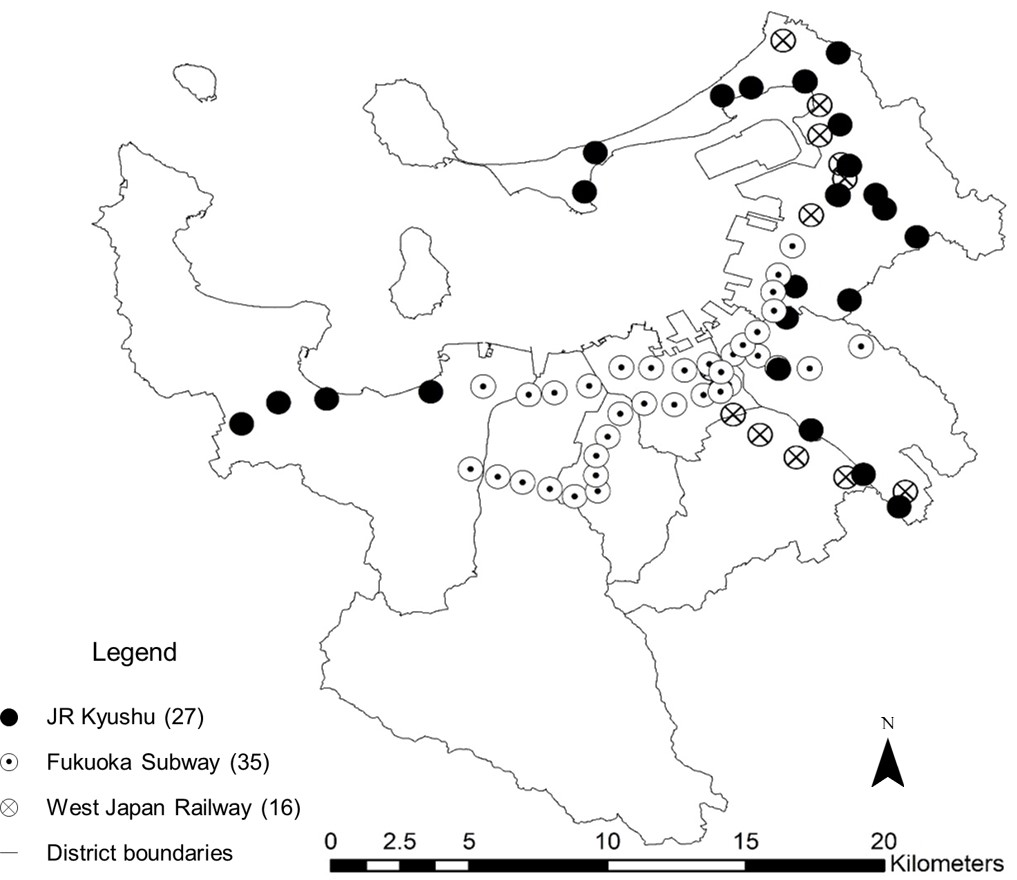
\includegraphics[width=1\linewidth]{fig1}}
\end{figure}

%
\begin{figure}[htp]
    \caption{Process of Data Cleaning}
    \label{fig:2}
    \centering
    \fbox{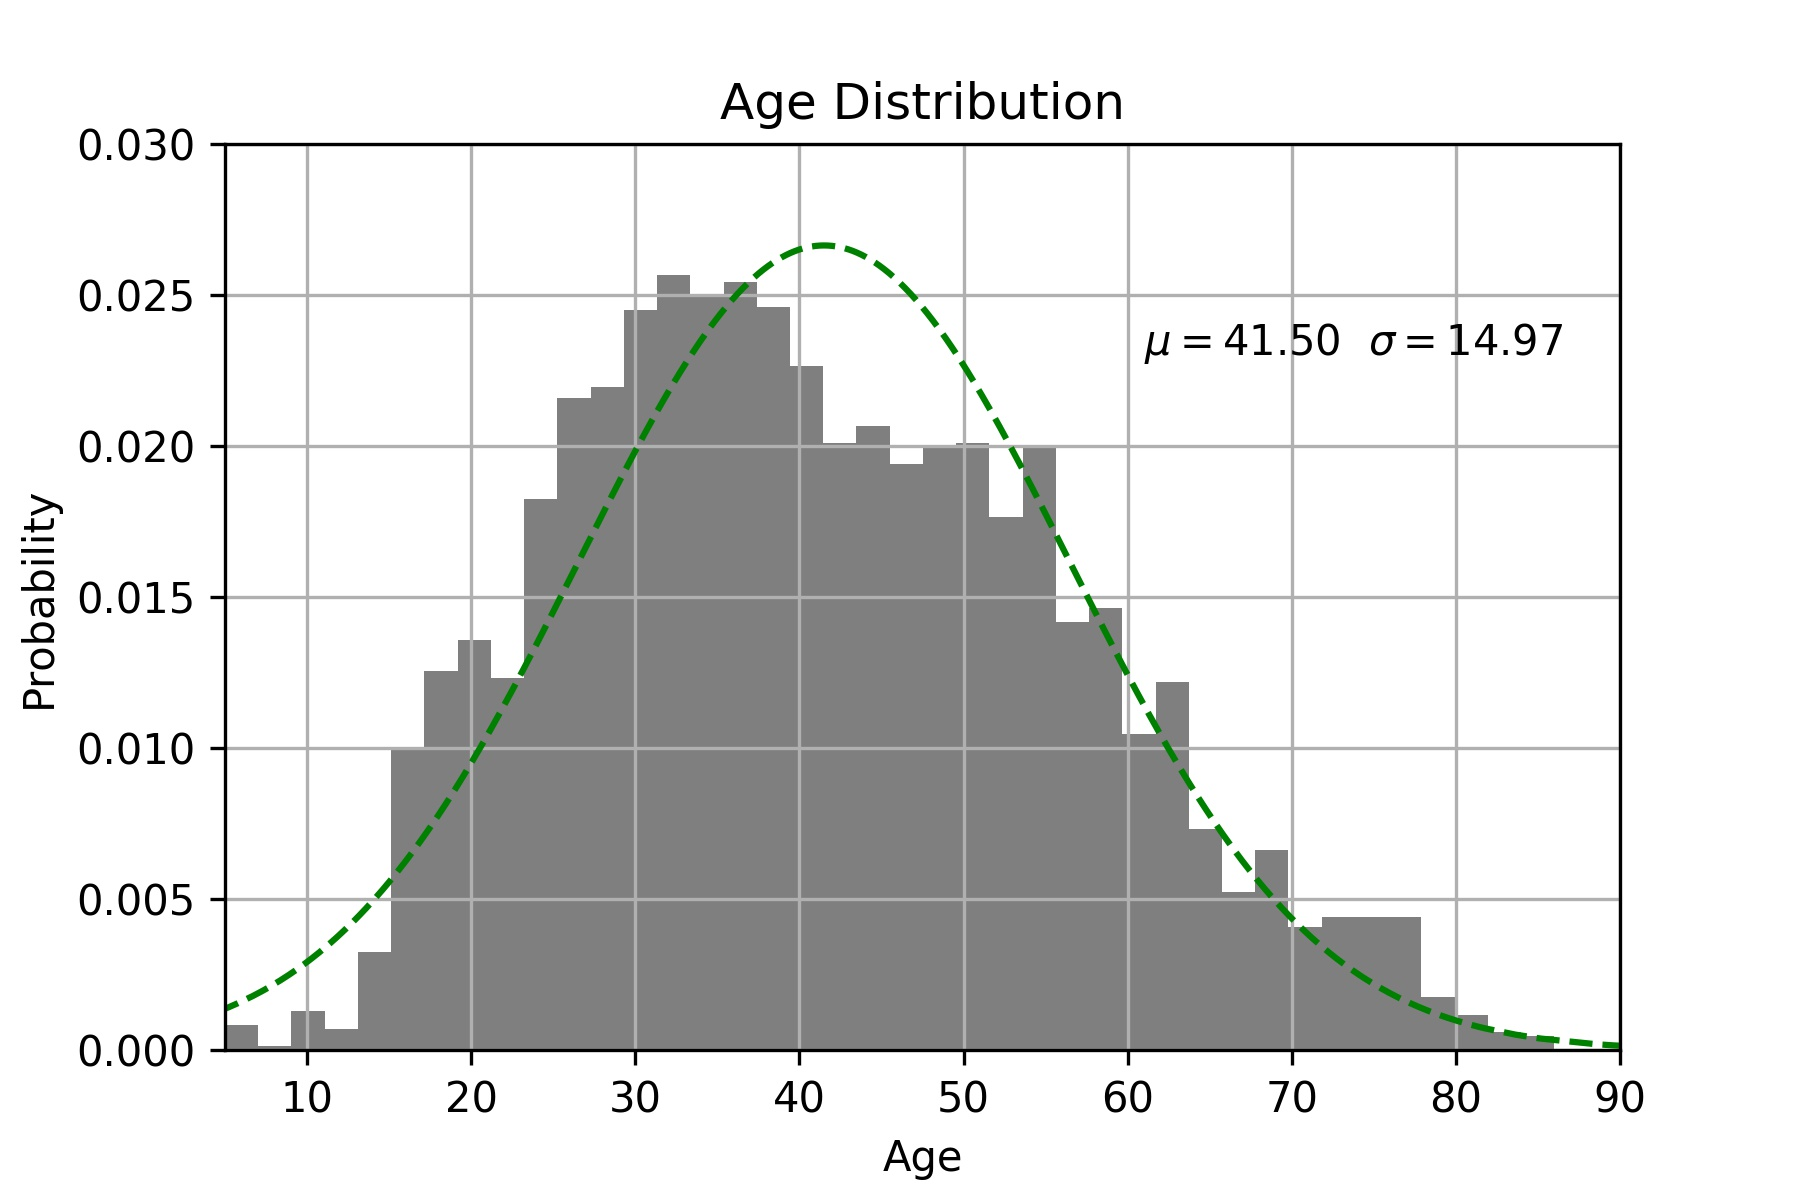
\includegraphics[width=1\linewidth]{fig2}}
\end{figure}

%
\begin{figure}[htp]
    \caption{The Age Distribution of Passengers}
    \label{fig:3}
    \centering
    \fbox{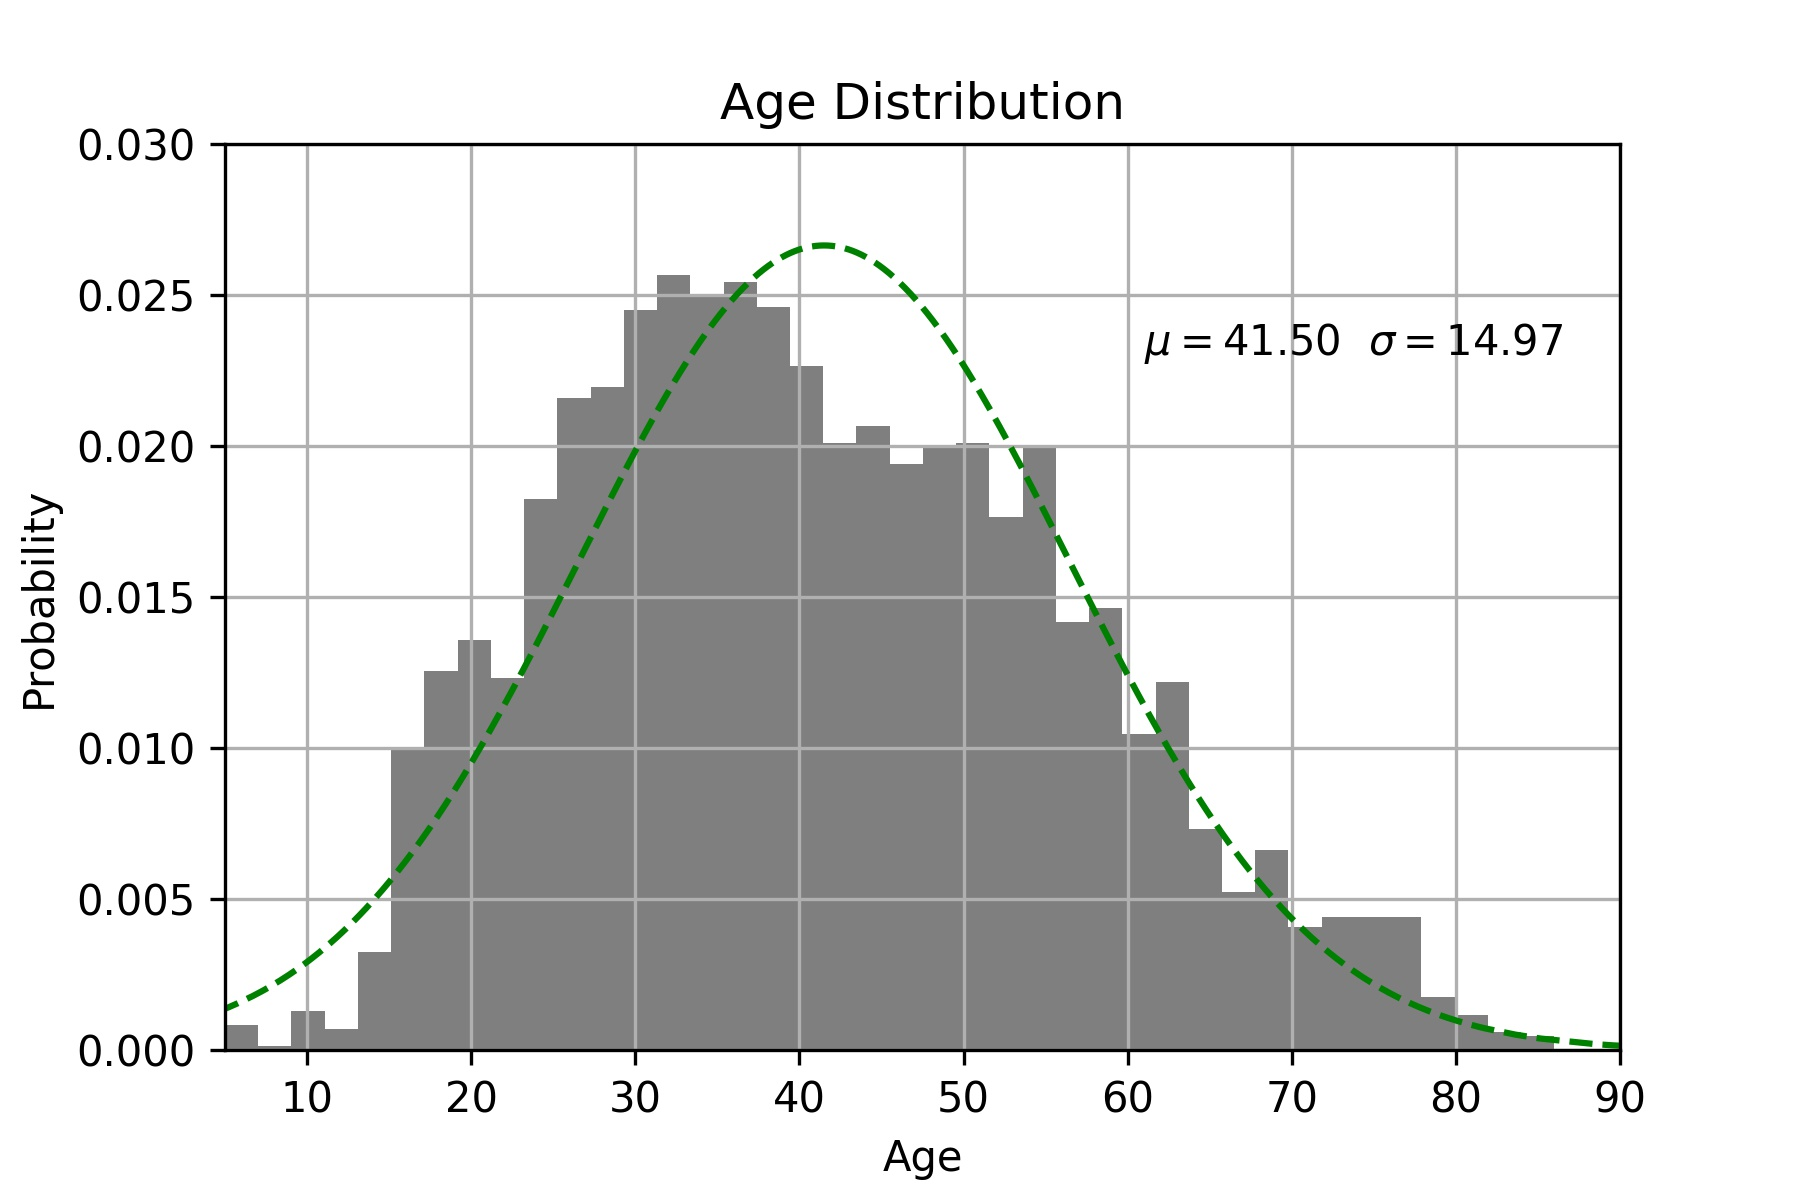
\includegraphics[width=1\linewidth]{fig3}}
\end{figure}

%
\begin{figure}[htp]
    \caption{Distribution of Walking Duration}
    \label{fig:4}
    \centering
    \fbox{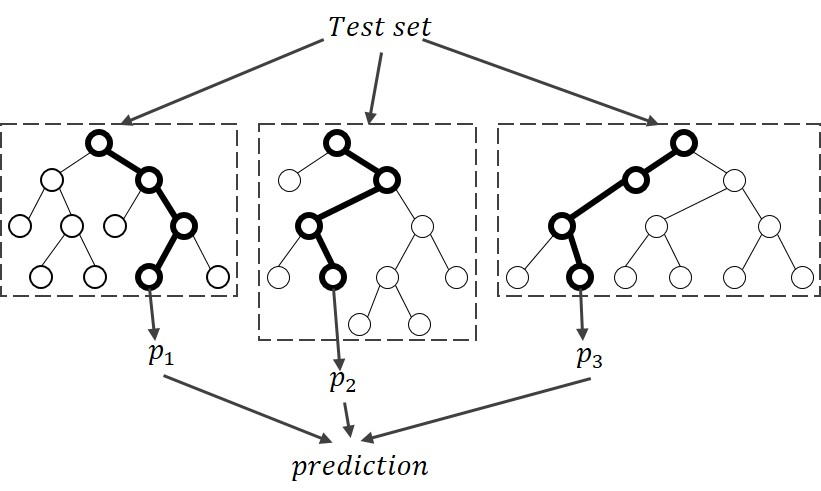
\includegraphics[width=1\linewidth]{fig4}}
\end{figure}

%
\begin{figure}[htp]
    \caption{Prediction Process in Random Forests Model}
    \label{fig:5}
    \centering
    \fbox{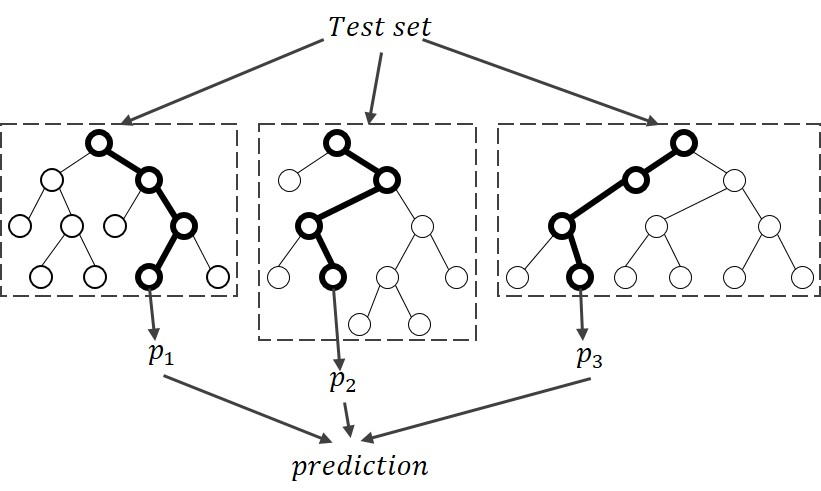
\includegraphics[width=1\linewidth]{fig5}}
\end{figure}

%
\begin{figure}[htp]
    \caption{Trend Line of Prediction and Test Set}
    \label{fig:6}
    \centering
    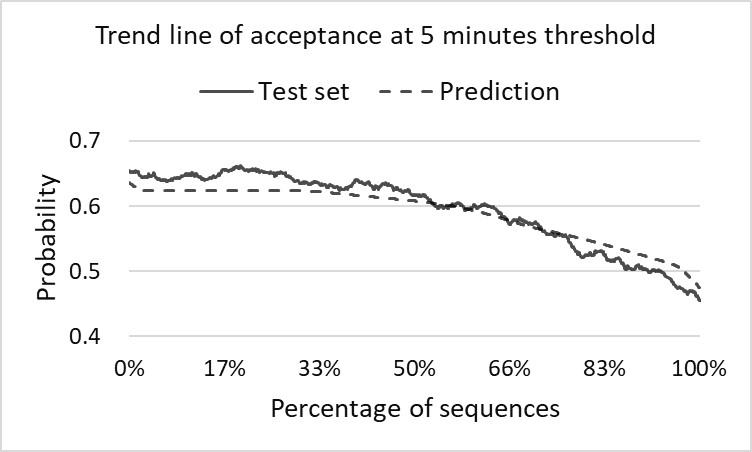
\includegraphics[width=0.7\linewidth]{fig6-1}\\
    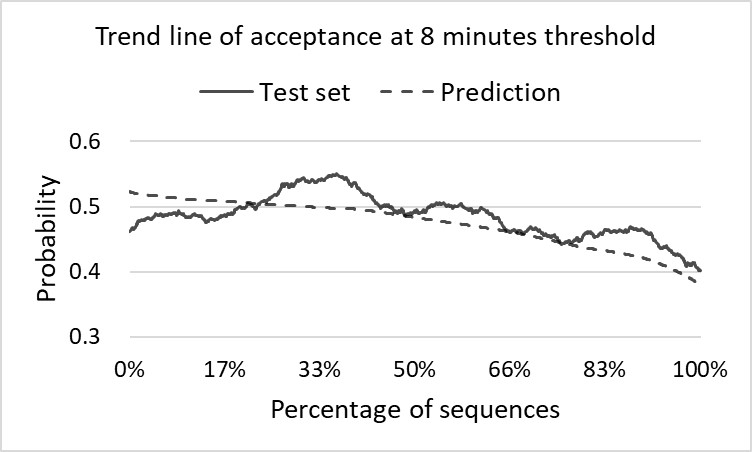
\includegraphics[width=0.7\linewidth]{fig6-2}\\
    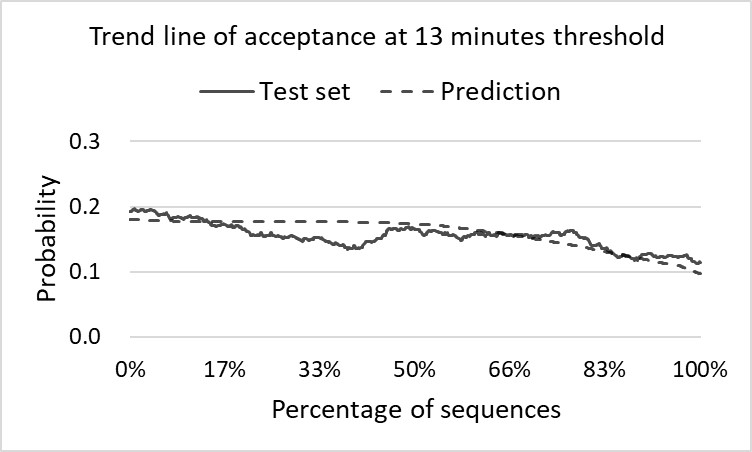
\includegraphics[width=0.7\linewidth]{fig6-3}\\
\end{figure}

% Format setting
\pagebreak

%
\bibliography{ascexmpl-new}

%
\end{document}
